

With the goal of finding the regime of hyper parameters and optimization techniques where multi-region demixing works best , we start with a series of experiment where we mixed known expression profiles in a controlled way. This allowed us to solve mulit-region demixing in a settings where the latent factors are known and used as a ground truth. We first describe how the dataset was created and then characterize how performance depends on the number of samples and the number of latent factors (cell types).

\subsubsection*{Creating the mixture dataset}
We created controlled mixtures from a set of real transcriptome measurements, measured using microarrays from isolated cells. \citet{okaty2011cell} have collected 195 cell-type-specific profiles from 64 cell types spanning multiple regions and layers of the mouse brain. These profiles were previously measured after isolating cell using varous tehcniques (FACS, LMD).
 
Specifically, we create the known latent factors by collecting profiles for the 3 major population of cell types in the brain: neurons, astrocytes and oligodendrocytes. Each profile $\c$ is represented by 14580 genes. Profiles were extracted from 7 brain regions:  cortex layer 5A, cortex layer 5B, cortex layer 6, striatum, cerebellum, brainstem and the spinal cord. For each of these region, we also found the proportions of the three cell types reported in the literature \cite{Herculano2014}. (cortex:  0.7,0.1,0.2 for neuron, astrocytes, oligodendrocytes; cerebellum: 0.5,0.15,0.35, other: 0.65,0.1,0.25).

To draw a mixture sample, we drew proportion values $p_{neuron},p_{astro},p_{oligo}$ by adding multiplicative noise to the literature proportions. Each proportion was multiplied by a random value in [0,1] and scaled back to a  sum of 1. Finally, we added multiplicative Gaussian noise to the expression level of all genes, of the form $N(1,\xi^2)$, with noise levels of $\xi=10\%$ and $\xi=1\% $.

We then used the known mixtures to test the quality of reconstructed profiles as a function of number of samples, noise level, number of factors, and the optimization algorithm. 



%We evaluated the reconstructed profiles by computing their %spearman correlation with the true profiles. We then, %matched the best true profiles to the reconstructed %profiles.

%Each time we sampled n noisy samples and reconstructed the %profiles using these samples. The error bars in figure  %represented the sem over 30 repetitions.  

We found that the use of priors was somewhat fragile. When we use priors that forced the demixed types to be close to the same profile types but that were gathered from different experiments the demixed

\subsubsection*{bench-marking optimization method for single region NMF}

Since NMF is a non-convex problem different optimization techniques often reach different local minimas. We tested if when initialized using the same starting points they will perform differently. We tested 4 optimization techniques and found that all performed better with more samples. When the number of sample is sufficiently large we did not observe much difference in the performance of the different methods. while in a small number of samples the block-pivoting and the active-set performed slightly better (both had the same level of performance) Figure \ref{fig:controlled_exp}(a).

\subsubsection*{analyzing number of samples}
We notice that in the regime of limited samples there is sweet spot where we benefit from using regularization over the naive cases. As we increase the number of samples the benefit that we gain by using our method diminishes Figure \ref{fig:controlled_exp}(b). With enough samples we solving the individual problems performs almost just as well. 



\begin{figure}[!hbt]
   (a) \hspace{120pt}(b) \hspace{120pt}(c) \hspace{120pt}
   \centering
     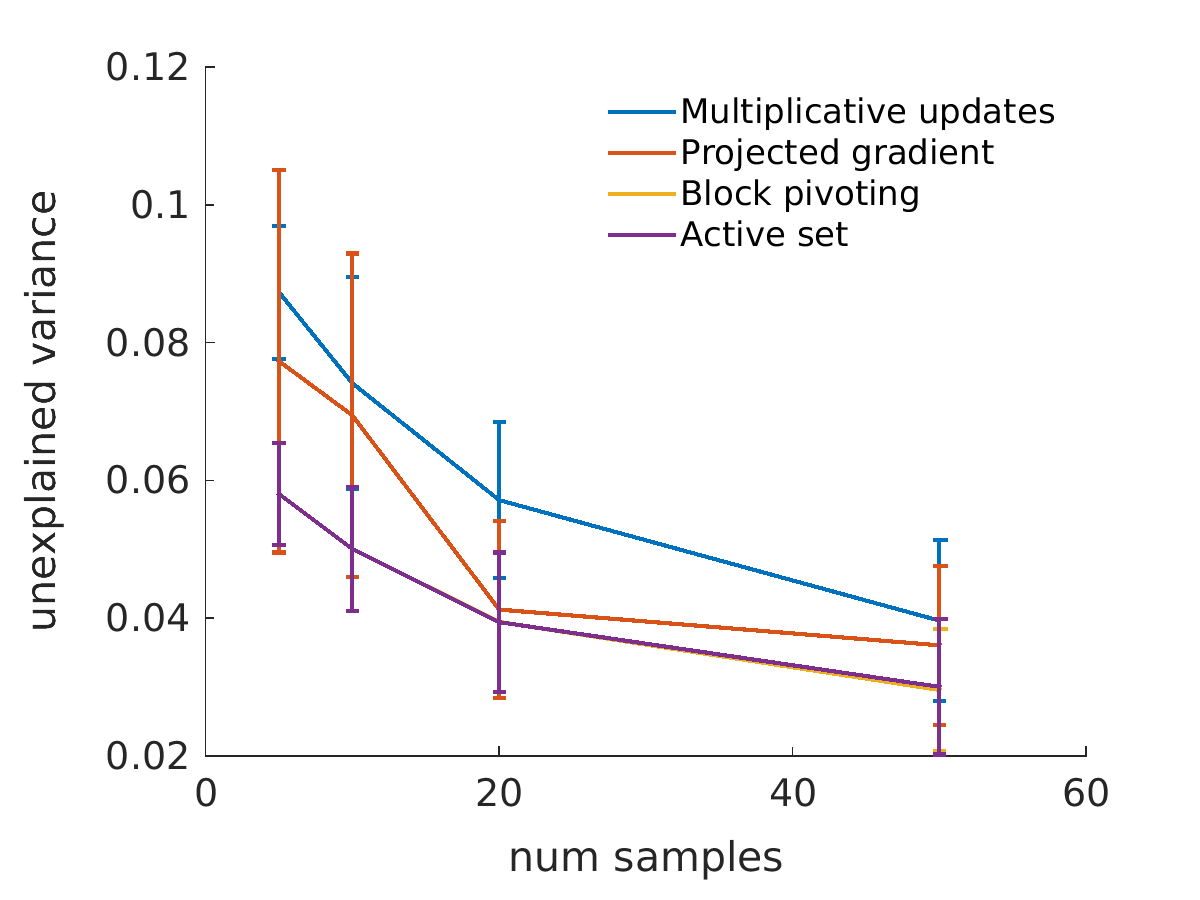
\includegraphics[width=0.32\textwidth]{methods}
     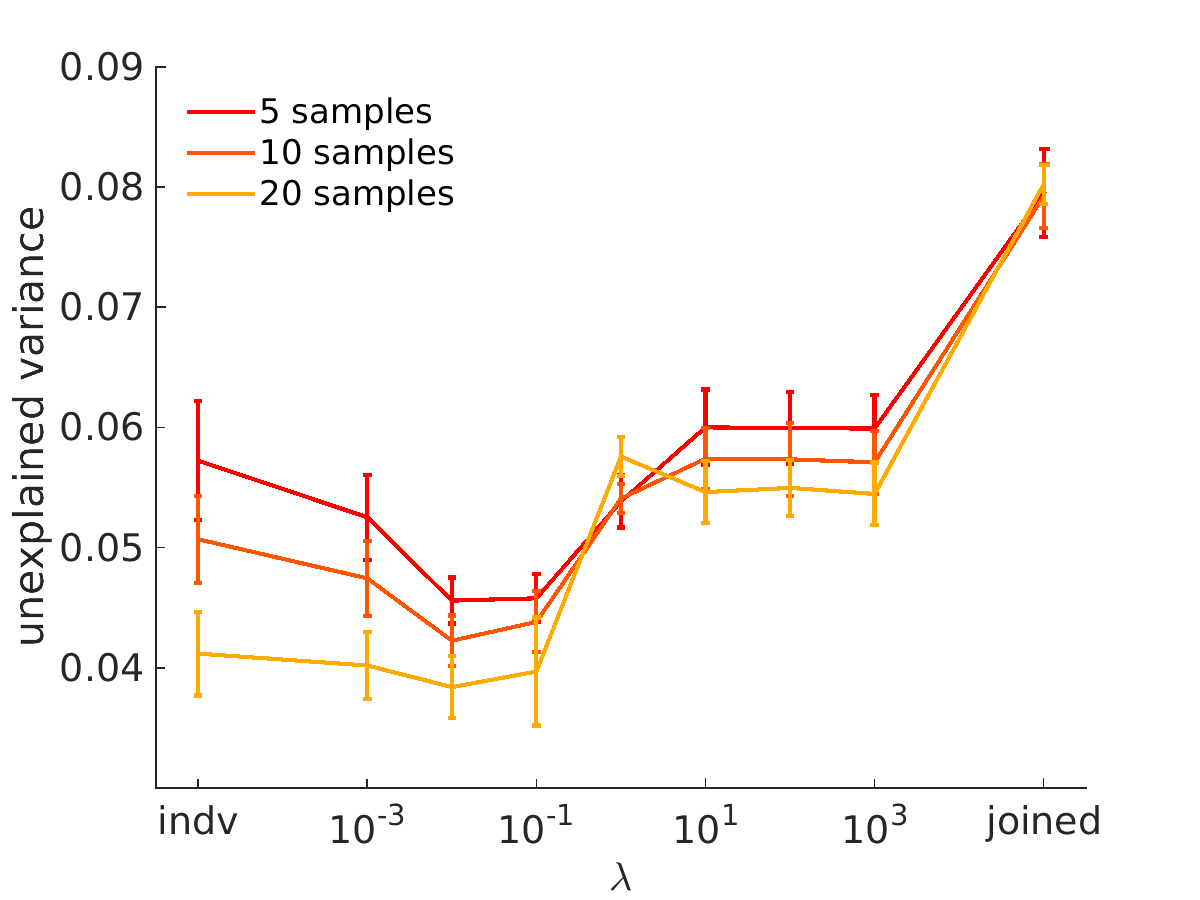
\includegraphics[width=0.32\textwidth]{lambda_sample_with20}
     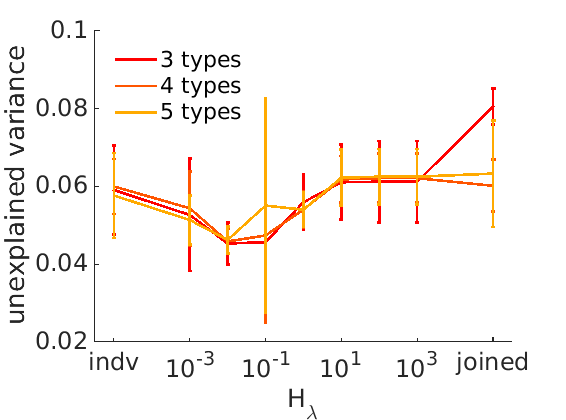
\includegraphics[width=0.32\textwidth]{num_types}
    \caption{Demixing in controlled experiments. 
    (a)  Within a single region, all optimization methods improve when using more samples. The {\em active set} approach and the {\em block pivoting} outperformed other methods, particularly with few samples. (b) Soft-sharing of latent factors lead to improved reconstruction in the multi-region settings, particularly with few samples. (c) Reconstruction using more cell types then needed does not improve the results.} 
    \label{fig:controlled_exp}
\end{figure}

{\bf{LIOR, HOW MANY REGIONS IN FIGURE 2B?        - 7}}



\subsubsection*{analyzing number of cell types}

As we increase the number of types the we are able to numerically better reconstruct the data matrix because we are allowing an approximation with of a larger rank. After we we perform the demixing we match the best demixed profiles with true profile. This can imporve the score since we can overfit. However, we did not notice any gain by using the extra profiles. It seems like it recovered the original profiles and some other vectors which helped to lower the overall fit but not the correlation to the original profiles. Overall it seems that this coincide with Ockham's razor and we can select simplest model which still capture the data \ref{fig:controlled_exp}(c). 



